%!TEX root = ../AutF3.tex
% -- Author: Phil Steinhorst, p.st@wwu.de
\chapter{Grundbegriffe}
\label{cha:property_T}
	Zu Beginn wollen wir die mathematischen Grundbegriffe einführen, die für die gesamte Arbeit essenziell sind. Zum einen werden wir $\cat$-Räume definieren und einen bekannten Satz zitieren, der uns in einigen Situationen die Existenz von Fixpunkten von Gruppenwirkungen liefern wird. Zum anderen definieren wir den Begriff des komplexen Hilbertraumes und zeigen erste Eigenschaften von Isometrien und affinen Abbildungen auf diesen, die besonders für das folgende Kapitel relevant sind. Mit einer Definition von Kazhdans Eigenschaft $\prT$ schließen wir letztlich dieses einführende Kapitel ab.

\section{CAT(0)-Räume}	
\label{sec:cat0}	
	Die folgenden Definitionen sind zusammengefasst entnommen aus \cite[Kap. 1]{Schwer}.
	
\begin{definition}[Geodäte, geodätischer Raum]
	Sei $(X,d)$ ein metrischer Raum und $x,y \in X$. Eine \textbf{Geodäte} von $x$ nach $y$ ist eine Abbildung $\gamma\colon [a,b] \rightarrow X$ mit $\gamma(a)=x$ und $\gamma(b) = y$ sowie $d(\gamma(s),\gamma(t)) = \abs{s-t}$ für alle $s,t \in [a,b]$. Wir schreiben kurz $\gamma\colon x \rightsquigarrow y$.
	
	Der Raum $(X,d)$ heißt \textbf{geodätisch}, wenn für alle $p,q \in X$ eine Geodäte $\gamma \colon p \rightsquigarrow q$ existiert.
\end{definition}

\begin{definition}[geodätisches Dreieck]
	Sei $(X,d)$ ein geodätischer Raum. Ein \textbf{geodätisches Dreieck} in $X$ ist ein Tupel $\Delta = (x,y,z,\alpha,\beta,\gamma)$ mit $x,y,z \in X$ und $\alpha\colon x \rightsquigarrow y, \beta\colon y \rightsquigarrow z, \gamma\colon z \rightsquigarrow x$. Die Geodäten $\alpha, \beta, \gamma$ heißen \textbf{Seiten} von $\Delta$.
\end{definition}

Ist $\Delta = (p,q,r,\alpha,\beta,\gamma)$ ein geodätisches Dreieck in $(X,d)$, so findet man unter Zuhilfenahme der Dreiecksungleichung stets drei Punkte $\tilde{p},\tilde{q},\tilde{r}$ und entsprechende Geodäten $\tilde{\alpha}, \tilde{\beta}, \tilde{\gamma}$ im euklidischen Raum $(\RR^2,d_2)$, sodass gilt:
\[
	d(p,q) = d_2(\tilde{p},\tilde{q}), \qquad d(q,r) = d_2(\tilde{q},\tilde{r}), \qquad d(r,p) = d_2(\tilde{r},\tilde p).
\]
Das geodätische Dreieck $(\tilde{p},\tilde{q},\tilde{r}, \tilde{\alpha}, \tilde{\beta}, \tilde{\gamma})$ heißt \textbf{Vergleichsdreieck} zu $\Delta$. Ist $v = \gamma(s) \in X$ für ein $s$, so heißt $\tilde{v} = \tilde{\gamma}(s) \in \RR^2$ \textbf{Vergleichspunkt} von $v$.

\begin{definition}[$\cat$-Raum]
	Sei $(X,d)$ ein metrischer Raum. Ein geodätisches Dreieck $\Delta$ in $X$ hat die $\mathbf{CAT(0)}$\textbf{-Eigenschaft}, wenn für alle Punkte $n,m$ auf den Seiten von $\Delta$ und ihre Vergleichspunkte $\tilde{n}, \tilde{m}$ auf den Seiten von $\tilde{\Delta}$ gilt:
	\[
		d(n,m) \leq d_2(\tilde{n},\tilde{m}).
	\]
	Ein geodätischer Raum $(X,d)$ heißt $\mathbf{CAT(0)}$\textbf{-Raum}, wenn alle Dreiecke in $X$ die $\cat$-Eigenschaft besitzen. 
\end{definition}

\begin{figure}[h]
	\centering
	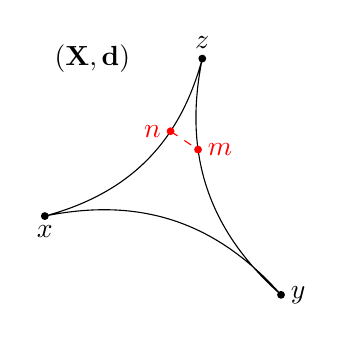
\begin{tikzpicture}[scale=1]
		\draw (0,1) node[fill,circle,inner sep=1pt]{}
			to [bend left] (3,0) node[fill,circle,inner sep=1pt]{} 
			to [bend left] coordinate[pos=.66] (M) (2,3) node[fill,circle,inner sep=1pt]{}
			to [bend left] coordinate[pos=.33] (N) cycle;
		\draw (0,1) node[below]{$x$};
		\draw (3,0) node[right]{$y$};
		\draw (2,3) node[above]{$z$};
		\draw (N) node[fill,circle,inner sep=1pt,color=red]{};
		\draw (N) node[left,color=red]{$n$};
		\draw (M) node[fill,circle,inner sep=1pt,color=red]{};
		\draw (M) node[right,color=red]{$m$};
		\draw[color=red, dashed] (N) -- (M);
		\draw (0,3) node[right]{$\mathbf{(X,d)}$};
	\end{tikzpicture} \hspace{2cm}
	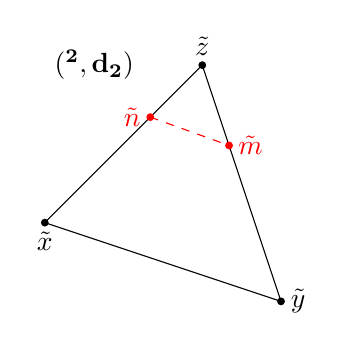
\begin{tikzpicture}[scale=1]
	\draw (0,1) node[fill,circle,inner sep=1pt]{}
	to (3,0) node[fill,circle,inner sep=1pt]{} 
	to coordinate[pos=.66] (M) (2,3) node[fill,circle,inner sep=1pt]{}
	to coordinate[pos=.33] (N) cycle;
	\draw (0,1) node[below]{$\tilde{x}$};
	\draw (3,0) node[right]{$\tilde{y}$};
	\draw (2,3) node[above]{$\tilde{z}$};
	\draw (N) node[fill,circle,inner sep=1pt,color=red]{};
	\draw (N) node[left,color=red]{$\tilde{n}$};
	\draw (M) node[fill,circle,inner sep=1pt,color=red]{};
	\draw (M) node[right,color=red,xshift=-.2]{$\tilde{m}$};
	\draw[color=red, dashed] (N) -- (M);
	\draw (0,3) node[right]{$\mathbf{(\RR^2,d_2)}$};
	\end{tikzpicture}	
	\caption{Anschaulich gesprochen sind Dreiecke in $\cat$-Räumen \enquote{mindestens so dünn} wie ihre Vergleichsdreiecke im euklidischen Raum.}
\end{figure}

\begin{beispiel}
	\mbox{} \\[-1.4cm]
	\begin{enumerate}[(i)]
		\item Der euklidische Raum $(\RR^n,d_2)$ sowie jeder Hilbertraum ist $\cat$, da sich die geodätischen Dreiecke isomorph in den $(\RR^2, d_2)$ abbilden lassen.
		\item Der Raum $(\RR^2,d_1)$ mit $d_1(x,y) := \abs{x_1-x_2} + \abs{y_1 - y_2}$ ist nicht $\cat$: In der folgenden Grafik ist $d_1(n,m) = 2$, aber $d_2(\tilde{n},\tilde{m}) = \sqrt{3}$.
	\end{enumerate}
\end{beispiel}
	
\begin{figure}[h]
	\centering
	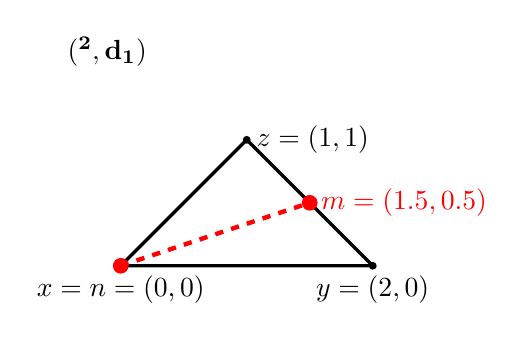
\begin{tikzpicture}[scale=1.6]	
		\draw (-1,0) node[below]{$x = n = (0,0)$};
		\draw (1,0) node[below]{$y = (2,0)$};
		\draw (0,1) node[right]{$z = (1,1)$};
		
		\draw[very thick] (-1,0) node[fill,circle,inner sep=2pt,color=red]{} -- (1,0) node[fill,circle,inner sep=1pt]{} -- coordinate[pos=.5] (M) (0,1) node[fill,circle,inner sep=1pt]{} -- cycle;
		
		\draw (M) node[fill,circle,inner sep=2pt,color=red]{};
		\draw (M) node[right,color=red,xshift=.6]{$m = (1.5,0.5)$};
		\draw[color=red,dashed,ultra thick] (-1,0) -- (M);
		\draw (-1.5,1.7) node[right]{$\mathbf{(\RR^2,d_1)}$};
	\end{tikzpicture} \hspace{1.5cm}
	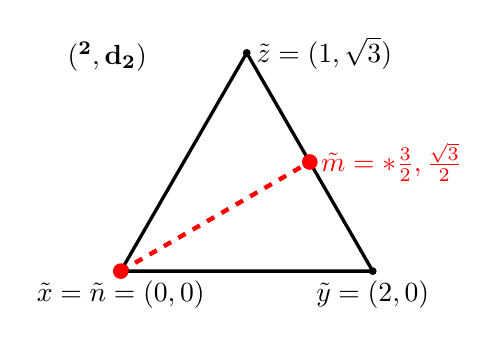
\begin{tikzpicture}[scale=1.6]	
		\draw[very thick] (0,0) node[fill,circle,inner sep=2pt,color=red]{} -- (2,0) node[fill,circle,inner sep=1pt]{} -- coordinate[pos=.5] (M) (1,1.732051) node[fill,circle,inner sep=1pt]{} -- cycle;
		
		\draw (0,0) node[below]{$\tilde{x} = \tilde{n} =(0,0)$};
		\draw (2,0) node[below]{$\tilde{y} = (2,0)$};
		\draw (1,1.732051) node[right]{$\tilde{z} = (1,\sqrt{3})$};
		
		\draw (M) node[fill,circle,inner sep=2pt,color=red]{};
		\draw (M) node[right,color=red,xshift=.6]{$\tilde{m} = \enbrace*{\frac{3}{2},\frac{\sqrt{3}}{2}}$};
		\draw[color=red,dashed,ultra thick] (0,0) -- (M);
		\draw (-0.5,1.7) node[right]{$\mathbf{(\RR^2,d_2)}$};	
	\end{tikzpicture}
	\caption{Der Raum $(\RR^2,d_1)$ ist nicht $\cat$.}
\end{figure}	
\newpage	
Ein für uns wesentliches Hilfsmittel ist der folgende Fixpunktsatz von \textsc{Bruhat} und \textsc{Tits}. Dieser sichert uns unter gewissen Bedingungen die Existenz eines globalen Fixpunktes, wenn eine Gruppe auf einen vollständigen $\cat$-Raum wirkt.

\begin{satz}[{\textsc{Bruhat-Tits}-Fixpunktsatz, vgl. \cite[Kor. II 2.8]{BridsonHaefliger}}]
	\label{satz_bruhat_tits}
	Sei $X$ ein vollständiger $\cat$-Raum, $G$ eine Gruppe und $\Phi\colon G \rightarrow \Isom(X)$ eine isometrische Gruppenwirkung von $G$ auf $X$. Dann sind folgende Aussagen äquivalent:
	\begin{enumerate}[(i)]
		\item $\Phi$ hat einen globalen Fixpunkt, das heißt es existiert ein $x \in X$ mit $\Phi(g)(x) = x$ für alle $g \in G$.
		\item Es existiert ein $x \in X$ mit beschränktem Orbit, das heißt $\Phi(G)(x) \subseteq X$ ist beschränkt.
		\item Jeder Orbit von $\Phi$ ist beschränkt.
	\end{enumerate}
\end{satz}	
	
\section{Hilberträume und Kazhdans Eigenschaft (T)}
\label{sec:prT}

\begin{definition}[Hilbertraum]
	Sei $\HH$ ein komplexer Vektorraum und $\sprod{\cdot,\cdot}\colon \HH \times \HH \rightarrow \CC$ ein \textbf{Skalarprodukt}, das heißt eine Abbildung mit folgenden Eigenschaften:
	\begin{enumerate}[(i)]
		\item $\sprod{\cdot,\cdot}$ ist sesquilinear, das heißt
		\begin{equation}
		\begin{aligned}
			\sprod{\lambda x + y,z} &= \overline{\lambda} \cdot \sprod{x,z} + \sprod{y,z} \\
			\sprod{x,\lambda y + z} &= \lambda \cdot \sprod{x,y} + \sprod{x,z}
		\end{aligned}
		\end{equation}
		für alle $\lambda \in \CC$ und $x,y,z \in \HH$.
		\item $\sprod{\cdot,\cdot}$ ist hermitesch, das heißt $\sprod{x,y} = \overline{\sprod{y,x}}$	für alle $x,y \in \HH$.
		\item $\sprod{\cdot,\cdot}$ ist positiv definit, das heißt $\sprod{x,x} \geq 0$ für alle $x \in \HH$ und $\sprod{x,x} = 0 \Leftrightarrow x = 0$.
	\end{enumerate}
	Dann induziert $\sprod{\cdot,\cdot}$ eine Norm und eine Metrik auf $\HH$ vermöge $\Norm{x} := \sqrt{\sprod{x,x}}$ und $d(x,y) := \Norm{x-y}$ für $x,y \in \HH$. Ist $(\HH,d)$ vollständig, so heißt $(\HH,\sprod{\cdot,\cdot})$ \textbf{Hilbertraum}.
\end{definition}

\begin{definition}[Isometrie]
	\label{def_isometrie}
	Sei $\HH$ ein Hilbertraum. Eine Abbildung $\varphi\colon \HH \rightarrow \HH$ heißt \textbf{Isometrie}, wenn für alle $x,y \in \HH$ gilt:
	\[ d(\varphi(x),\varphi(y)) = d(x,y). \]
	Wie auch für metrische Räume bezeichnen wir mit $\Isom(\HH) := \{\varphi \colon \HH \rightarrow \HH : f \text{ ist isometrisch}$ $\text{und bijektiv}\}$ die \textbf{Isometriegruppe} von $\HH$.
\end{definition}	
	
\begin{bemerkung}
	Für eine Isometrie $\varphi \colon \HH \rightarrow \HH$ gelten die Identitäten $\Norm{\varphi(x)-\varphi(y)} = \Norm{x-y}$ und $\sprod{\varphi(x)-\varphi(y),\varphi(x)-\varphi(y)}=\sprod{x-y,x-y}$ für alle $x,y \in \HH$.
\end{bemerkung}	

Als weiteres Hilfsmittel für die Arbeit mit Isometrien führen wir den Begriff der affinen Abbildung ein und zitieren den Satz von \textsc{Mazur} und \textsc{Ulam} über surjektive Isometrien. Aus letzterem folgt eine Aussage über die Struktur der Fixpunktmenge einer bijektiven Isometrie.

\begin{definition}[affine Abbildung]
\label{def_affine_abb}
	Sei $V$ ein reeller normierter Vektorraum. Eine Abbildung $f\colon V \rightarrow V$ heißt \textbf{affin}, wenn eine der folgenden äquivalenten Bedingungen erfüllt ist:
	\begin{enumerate}[(i)]
		\item Die Abbildung $x \mapsto f(x) - f(0)$ ist linear.
		\item Für alle $x,y \in V$ gilt $f\enbrace*{\frac{1}{2}(x+y)} = \frac{1}{2}(f(x)+f(y))$.
		\item Für alle $x,y \in V$ und $t \in [0,1]$ gilt $f((1-t)x + ty) = (1-t)f(x) + tf(y)$.
		\item Sind $v_1,\dots,v_n \in V$ und $\lambda_1,\dots,\lambda_n \in \RR$ mit $\sum_{i=1}^{n} \lambda_i = 1$, so gilt
		\[
			f\enbrace*{\sum\limits_{i=1}^{n} \lambda_i v_i} = \sum\limits_{i=1}^{n} \lambda_i f(v_i).
		\]
	\end{enumerate}
\end{definition}

\begin{beweis}
	Zur Äquivalenz von (i), (ii) und (iii) siehe  \cite{Jussi}. Die Implikation (iv) $\Rightarrow$ (iii) ist klar (Fall $n=2$). Wir zeigen mittels Induktion, dass auch (iv) aus (iii) folgt: Der Induktionsanfang $n=2$ entspricht gerade der Aussage (iii). Gelte also (iv) für ein festes $n \in \NN$. Dann gilt für $v_1, \dots, v_{n+1} \in V$ und $\lambda_1, \dots, \lambda_{n+1} \in \RR$ mit $\sum_{i=1}^{n+1} \lambda_i = 1$ und ohne Einschränkung $\lambda_{n+1} \neq 1$:
	\begin{equation}
	\begin{aligned}
		f \enbrace*{\sum\limits_{i=1}^{n+1} \lambda_i v_i} = \; &f\enbrace*{ (1-\lambda_{n+1}) \cdot \frac{1}{1-\lambda_{n+1}} \cdot \sum\limits_{i=1}^{n} \lambda_i v_i + \lambda_{n+1} v_{n+1}} \\
		\overset{\text{(iii)}}{=} \; &(1-\lambda_{n+1}) \cdot f \enbrace*{\frac{1}{1-\lambda_{n+1}} \cdot \sum\limits_{i=1}^{n} \lambda_i v_i} + \lambda_{n+1} f(v_{n+1}) \\
		= \; &(1-\lambda_{n+1}) \cdot f\enbrace*{\sum\limits_{i=1}^{n} \frac{\lambda_i}{1-\lambda_{n+1}} v_i} + \lambda_{n+1} f(v_{n+1})
	\end{aligned}
	\end{equation}
	Nun ist
	\[
		\sum\limits_{i=1}^{n} \frac{\lambda_i}{1-\lambda_{n+1}} = \sum\limits_{i=1}^{n} \frac{\lambda_i}{\sum\limits_{k=1}^{n} \lambda_k} = 1,
	\]
	also ist die Induktionsvoraussetzung anwendbar und wir erhalten weiter:
	\begin{equation}
	\begin{aligned}
		&(1-\lambda_{n+1}) \cdot f\enbrace*{\sum\limits_{i=1}^{n} \frac{\lambda_i}{1-\lambda_{n+1}} v_i} + \lambda_{n+1} f(v_{n+1}) \\
		\overset{\text{I.V.}}{=} \; &(1-\lambda_{n+1}) \cdot \sum\limits_{i=1}^{n} \frac{\lambda_i}{1-\lambda_{n+1}} f(v_i) + \lambda_{n+1} f(v_{n+1}) \\
		= \; &\sum\limits_{i=1}^{n+1} \lambda_i f(v_i).
	\end{aligned}
	\end{equation}
	Somit gilt (iv) für alle $n \in \NN$. \qedhere
	
\end{beweis}

\begin{satz}[\textsc{Mazur-Ulam}, \cite{Jussi}]
\label{satz_mazur-ulam}
	Sei $f\colon \HH \rightarrow \HH$ eine bijektive Isometrie auf einem reellen Hilbertraum $\HH$. Dann ist $f$ affin.
\end{satz}

\begin{korollar}
\label{kor:fix_affin}
	Sei $\HH$ ein reeller Hilbertraum und $\varphi \in \Isom(\HH)$. Ist die Fixpunktmenge $\Fix(\varphi) := \{x \in \HH : \varphi(x) = x\}$ von $\varphi$ nicht leer, so ist $\Fix(\varphi)$ ein affiner Unterraum von $\HH$.
\end{korollar}

\begin{beweis}
	Sei $\xi \in \Fix(\varphi) \neq \emptyset$. Nach Satz~\ref{satz_mazur-ulam} ist $\varphi(x) = L(x) + b$ für alle $x \in \HH$ mit $L\colon \HH \rightarrow \HH$ linear und $b \in \HH$. Also gilt $\varphi(\xi) = L(\xi) + b = \xi$ bzw. $L(\xi) = \xi - b$.
	
	Wir zeigen nun, dass $\Fix(\varphi) = \xi + \Eig(1,L)$ gilt, wobei $\Eig(1,L)$ der Eigenraum von $L$ zum Eigenwert $1$ ist.	
	\begin{description}
		\item["$\subseteq$":] Sei $x \in \Fix(\varphi)$, also $\varphi(x) = L(x) + b = x$. Dann ist
		\[
		L(x-\xi) = L(x) - L(\xi) = (x-b) - (\xi - b) = x - \xi.
		\]
		Also ist $x - \xi \in \Eig(1,L)$ und somit $x \in \xi + \Eig(1,L)$.
		\item["$\supseteq$":] Sei $x \in \xi + \Eig(1,L)$, das heißt $x = \xi + v$ mit $L(v) = v$. Dann ist
		\[
		\varphi(x) = L(x) + b = L(\xi) + L(v) + b = \xi - b + v + b = \xi + v = x.
		\]
		Also ist $x \in \Fix(\varphi)$. \qedhere
	\end{description} 
\end{beweis}

Obschon wir in den folgenden Kapiteln äquivalente Formulierungen nutzen werden, möchten wir der Vollständigkeit halber die ursprüliche Definition der Kazhdan-Eigenschaft $\prT$ nach \cite[Def. 1.1.3]{BekkaHarpeValette} angeben. Diese ist definiert mit Hilfe von unitären Darstellungen topologischer Gruppen auf komplexen Hilberträumen.

\begin{definition}[unitäre Gruppe]
	Sei $\HH$ ein komplexer Hilbertraum. Eine lineare Abbildung $f\colon \HH \rightarrow \HH$ heißt \textbf{unitär}, falls $\sprod{f(x),f(y)} = \sprod{x,y}$ für alle $x,y \in \HH$ gilt. Wir nennen
	\[
		\UU(\HH) := \{f \colon \HH \rightarrow \HH : f \text{ ist unitär und bijektiv}\}
	\]
	die \textbf{unitäre Gruppe} von $\HH$.
\end{definition}

\begin{definition}[unitäre Darstellung]
	Sei $G$ eine topologische Gruppe. Eine \textbf{unitäre Darstellung} $(\pi,\HH)$ von $G$ auf einem komplexen Hilbertraum $\HH$ ist ein Gruppenhomomorphismus $\pi \colon G \rightarrow \UU(\HH)$, sodass die Abbildung
	\begin{equation}
	\begin{aligned}
		G &\longrightarrow \HH \\
		g &\longmapsto \pi(g)(x)
	\end{aligned}
	\end{equation}
	stetig ist für alle $x \in \HH$.
\end{definition}

\begin{definition}
	Sei $G$ eine topologische Gruppe und $(\pi,\HH)$ eine unitäre Darstellung.
	\begin{enumerate}[(i)]
		\item Sei $Q \subseteq G$ und $\varepsilon > 0$. Ein Vektor $x \in \HH$ heißt $\bm{(Q,\varepsilon)}$\textbf{-invariant}, wenn gilt
		\[
			\sup_{g \in Q} \ \Norm{\pi(g)(x) - x} \le \varepsilon \cdot \Norm{x}.
		\]
		\item Wir sagen, $(\pi,\HH)$ hat \textbf{invariante Vektoren}, falls ein $x \in \HH \setminus \setzero$ existiert, sodass für alle $g \in G$ gilt: $\pi(g)(x) = x$.
	\end{enumerate}
\end{definition}

\begin{definition}[Kazhdans Eigenschaft $\prT$]
	Eine topologische Gruppe $G$ hat \textbf{Kazhdans Eigenschaft (T)}, wenn eine kompakte Menge $Q \subseteq G$ und ein $\varepsilon > 0$ existiert, sodass gilt: Jede unitäre Darstellung von $G$, die einen $(Q,\varepsilon)$-invarianten Vektor besitzt, hat auch einen invarianten Vektor.
\end{definition}

\cleardoubleoddemptypage